\documentclass{standalone}
\usepackage{tikz}
\begin{document}
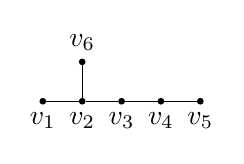
\begin{tikzpicture}[every node/.style={draw, circle, fill=black, minimum size=2pt, inner sep=0pt}]
\node[fill=black, label=below:{$v_{1}$}] (G1N2) at (6,5) {};
\node[fill=black, label=below:{$v_{2}$}] (G1N0) at (6.5,5) {};
\node[fill=black, label=below:{$v_{3}$}] (G1N1) at (7,5) {};
\node[fill=black, label=below:{$v_{4}$}] (G1N4) at (7.5,5) {};
\node[fill=black, label=below:{$v_{5}$}] (G1N5) at (8,5) {};
\node[fill=black, label=above:{$v_{6}$}] (G1N3) at (6.5,5.5) {};
\draw (G1N0) -- (G1N1);
\draw (G1N0) -- (G1N2);
\draw (G1N0) -- (G1N3);
\draw (G1N1) -- (G1N4);
\draw (G1N4) -- (G1N5);
\end{tikzpicture}
\end{document}
